\documentclass[tikz,border=20pt]{standalone}
\usepackage{amsmath,amssymb}
\usepackage{tikz}
\usetikzlibrary{arrows.meta,calc}

\begin{document}
	
	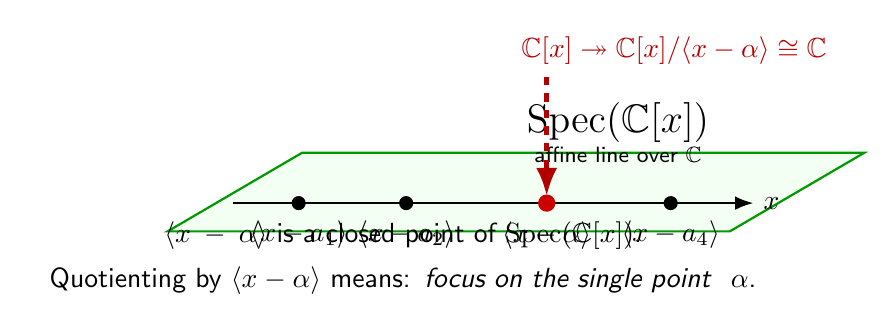
\begin{tikzpicture}[
		x={(1cm,0cm)},
		y={(0.65cm,0.38cm)},
		z={(0cm,1.7cm)},
		scale=1.05,
		font=\sffamily,
		>=Latex,
		pt/.style={circle, fill=black, inner sep=1.8pt},
		sel/.style={circle, fill=red!80!black, inner sep=2.2pt}
		]
		
		% Main plane
		\draw[fill=green!5, draw=green!60!black, thick]
		(-3.2,-0.7,0) -- (3.6,-0.7,0) -- (3.6,1.8,0) -- (-3.2,1.8,0) -- cycle;
		
		\node[align=center] at (0.2,2.45,0)
		{\Large $\operatorname{Spec}(\mathbb{C}[x])$\\[-1pt]\footnotesize affine line over $\mathbb C$};
		
		% x-axis
		\draw[->, thick] (-3.0,0.2,0) -- (3.3,0.2,0) node[right] {$x$};
		
		% several visible points
		\node[pt, label=below:{$\langle x-a_1\rangle$}] at (-2.2,0.2,0) {};
		\node[pt, label=below:{$\langle x-a_2\rangle$}] at (-0.9,0.2,0) {};
		\node[sel, label=below:{$\langle x-\alpha\rangle$}] at (0.8,0.2,0) {};
		\node[pt, label=below:{$\langle x-a_4\rangle$}] at (2.3,0.2,0) {};
		
		% quotient label
		\draw[->, ultra thick, dashed, red!70!black] (0.8,0.2,0.9) -- (0.8,0.2,0.05);
		\node[align=center, text=red!70!black] at (1.95,0.8,0.95)
		{$\mathbb C[x]\twoheadrightarrow \mathbb C[x]/\langle x-\alpha\rangle\cong \mathbb C$};
		
		% caption
		\node[align=center, text width=9.3cm] at (0.2,-1.55,0)
		{$\displaystyle \langle x-\alpha\rangle$ is a closed point of $\operatorname{Spec}(\mathbb C[x])$.\\[4pt]
			Quotienting by $\langle x-\alpha\rangle$ means: \emph{focus on the single point } $\alpha$.};
		
	\end{tikzpicture}
	
\end{document}